% Midterm section: RQ2 spike results (owner: Lordphone Wen). Draft for Shirley to merge.
% Figure: experiments/spike/results/20261103-rtx5090/recovery.png
% Numbers: experiments/spike/results/20261103-rtx5090/summary.md (medians of 5 runs).

\section{Preliminary Results: Recovery Cost by Fault Domain}
\label{sec:spike}

\textbf{Setup.} We ran a one-day spike to size RQ2 before building the recovery paths. It uses one NVIDIA RTX~5090 (32~GB, Blackwell), the pinned vLLM~0.32.0 container, and Qwen3-4B in BF16 with a 32K context limit. The GPU platform moved from PSC to this local machine on 2026-11-03, and its results are reported on their own. A stdlib-only harness emits every interval boundary as a schema-validated telemetry event; all 2{,}598 events in the run pass the schema check. Each cell is the median of five runs, and $\sigma$ is below 2\% unless noted; the empty-JIT-cache cold start is a single first-start observation ($n{=}1$) and is diagnostic only. A scripted 10-step agent loop (8K-token prefix, 128 generated and 256 tool tokens per step) is killed with \texttt{SIGKILL} after 64 tokens of step~6. The killed process is either the runner or the vLLM inference process. Automatic prefix caching (APC) is a factor.

\begin{table}[ht]
\caption{Spike measurements on one RTX~5090 (medians of 5 runs; $^\dagger$single run).}
\label{tab:spike}
\vskip 0.10in
\centering
\small
\begin{tabular}{@{}lr@{}}
\toprule
Measurement & Result \\
\midrule
Cold start, warm caches & 20.5~s \\
Cold start, empty JIT cache$^\dagger$ & 86~s \\
Prefill 2K / 8K / 16K & 0.09 / 0.45 / 1.09~s \\
Prefill 16K, APC hit & 0.042~s \\
Decode, single stream & 161~tok/s \\
\midrule
Inference kill $\to$ next token & 21.6~s \\
Runner kill, APC off / on & 0.63 / 0.073~s \\
\bottomrule
\end{tabular}
\vskip -0.05in
\end{table}

\begin{figure}[ht]
\centering
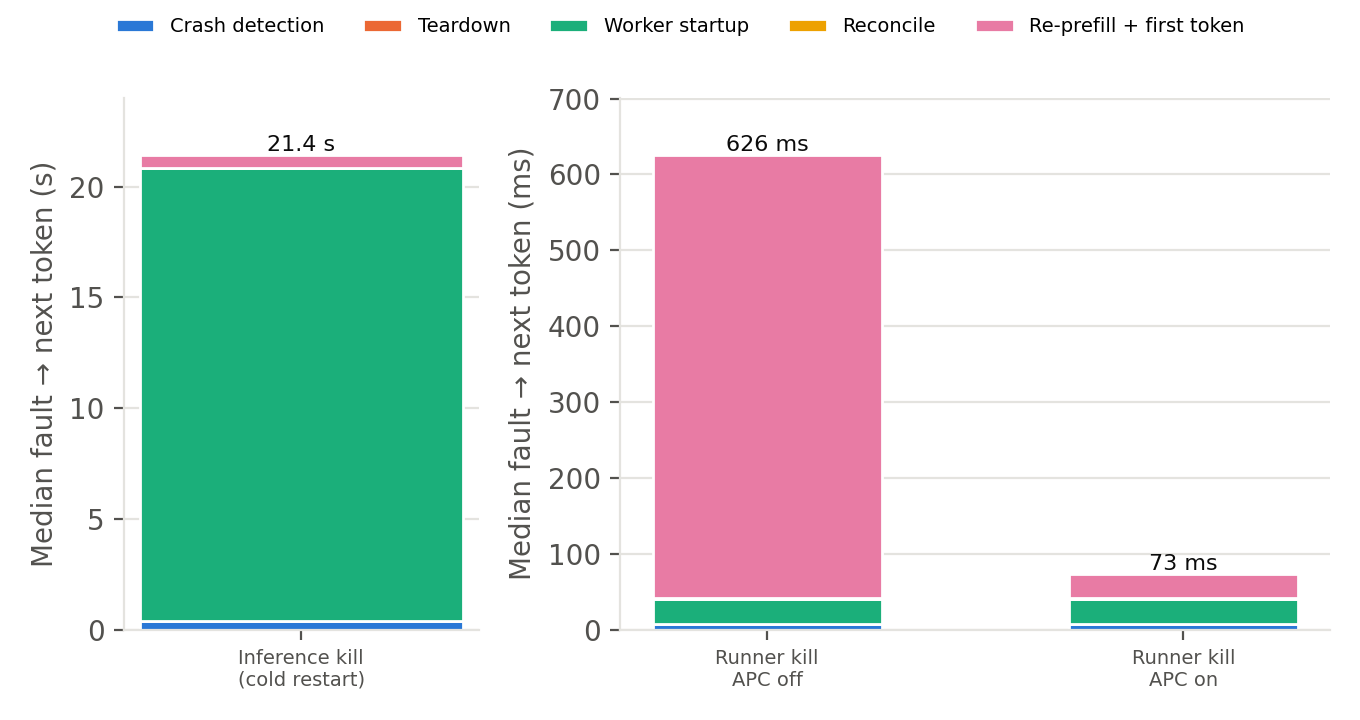
\includegraphics[width=\columnwidth]{figures/recovery.png}
\caption{Median fault-to-next-token time by fault domain, split into detection, teardown, worker startup, log reconciliation, and re-prefill plus first token. Note the different scales: the inference-process panel is in seconds and the runner panel in milliseconds.}
\label{fig:recovery}
\end{figure}

\textbf{Worker startup dominates inference-process recovery.} After an inference crash, 95\% of the 21.6~s until the next token is spent starting a replacement vLLM worker. Re-prefilling the 10K-token committed prefix takes only 0.6~s. Even with every cache warm, a cold start costs 19$\times$ a 16K-token prefill. In the single first start we observed on a new host it cost 79$\times$, because the image has no native sm\_120 kernels and the CUDA driver JIT-compiles their PTX for about 65~s. Under the current single-GPU process-restart scope, startup is therefore the term that recovery-time results must report and break out. A replacement worker that is already loaded would remove it; warm-replica failover is not implemented or measured here and remains future work.

\textbf{Runner crashes cost re-prefill, and APC decides how much.} When only the runner dies, the GPU worker survives. Recovery is 625~ms with APC off, 93\% of it re-prefill, and 73~ms with APC on, because the committed prefix is still cached (vLLM reports a hit on all but the final partial 16-token block). Replaying the durable log takes about 1~ms. Because APC changes runner-crash recovery by 8.5$\times$ and repeated-prefix prefill by up to 26$\times$, APC is a factor that every RQ2 result must report, never a fixed setting. The APC-off arm isolates pure re-prefill cost.

\textbf{Lost decode is expensive.} Single-stream decode runs at 161~tok/s, about 100$\times$ slower per token than prefill (15--23K~tok/s). Thinking mode more than doubles answer length on our agent prompts, from a median of 660 to 1{,}598 tokens, which is about 10~s of decode. A full restart at step~6 would redo about 4~s of decode for the five completed steps, before counting tool calls. Resume replaces this with 0.6~s of re-prefill. Tokens decoded in the step that crashed are still lost; checkpointing them is not implemented here and remains future work.

\textbf{Reproducibility notes.} The pinned image crashes at import because it bundles a CUDA~13 build of \texttt{torchcodec}. We mount a shim that makes the import fail cleanly; the image itself is unchanged. All restart measurements state whether the driver JIT, torch.compile, and Triton caches were warm. Under load the GPU held a median SM clock of 2{,}850~MHz and peaked at 81\,$^\circ$C, with no thermal throttling.

\textbf{Next.} For the main experiments we will move to $\ge$20 runs per cell with paired seeds, keep the single-GPU process-restart setup, and report APC on and off side by side. Reconciliation will use the real tool service's \texttt{query(op\_id)} instead of a local log replay. Warm-replica failover (which on this machine would share the single GPU with the primary) and decode checkpointing are future work beyond the current scope.
